\documentclass[]{article}
\usepackage{beamerarticle}
\usepackage[utf8]{inputenc}
\usepackage{hyperref}
\hypersetup{%
  colorlinks=true,% hyperlinks will be coloured
  citecolor={blue!50!black},
  urlcolor={blue!80!black},
  linkcolor=blue,% hyperlink text will be green
  linkbordercolor=blue,% hyperlink border will be red
}

% Math
\usepackage{amssymb,amsmath,amsthm} 
\theoremstyle{plain} % other formats: definition, plain, remark
\newtheorem{proposition}{Proposition}
\newtheorem{define}{Definition}

% Fontfamily
\usepackage{times}%\usepackage{palatino,lmodern, times}

% Page settings
\usepackage[letterpaper, margin=1in]{geometry}
\usepackage{setspace}                           
\onehalfspacing %\doublespacing  % \singlespacing 

% Appendix
\usepackage{appendix}

% Line numbers
%\usepackage{lineno}
%\linenumbers


% Tables
\usepackage{dcolumn}
\usepackage{array,booktabs,longtable,rotating}
\newenvironment{tablenotes}[1][]{
  \begin{minipage}{\textwidth}\emph{Notes:}{\footnotesize #1}
}{\end{minipage}}
\makeatletter
\def\fps@table{htbp}
\makeatother

% Graphics
\usepackage{graphicx,grffile}
\makeatletter
\def\maxwidth{\ifdim\Gin@nat@width>\linewidth\linewidth\else\Gin@nat@width\fi}
\def\maxheight{\ifdim\Gin@nat@height>\textheight\textheight\else\Gin@nat@height\fi}
\makeatother
% Scale images if necessary, so that they will not overflow the page
% margins by default, and it is still possible to overwrite the defaults
% using explicit options in \includegraphics[width, height, ...]{}
\setkeys{Gin}{width=\maxwidth,height=\maxheight,keepaspectratio}
% set default figure placement to htbp
\makeatletter
\def\fps@figure{htbp}
\makeatother

\usepackage{natbib}% plainnat
\bibliographystyle{aer}
\usepackage{color}
\usepackage{fancyvrb}
\newcommand{\VerbBar}{|}
\newcommand{\VERB}{\Verb[commandchars=\\\{\}]}
\DefineVerbatimEnvironment{Highlighting}{Verbatim}{commandchars=\\\{\}}
% Add ',fontsize=\small' for more characters per line
\usepackage{framed}
\definecolor{shadecolor}{RGB}{255,255,255}
\newenvironment{Shaded}{\begin{snugshade}}{\end{snugshade}}
\newcommand{\KeywordTok}[1]{\textcolor[rgb]{0.12,0.11,0.11}{\textbf{#1}}}
\newcommand{\DataTypeTok}[1]{\textcolor[rgb]{0.00,0.34,0.68}{#1}}
\newcommand{\DecValTok}[1]{\textcolor[rgb]{0.69,0.50,0.00}{#1}}
\newcommand{\BaseNTok}[1]{\textcolor[rgb]{0.69,0.50,0.00}{#1}}
\newcommand{\FloatTok}[1]{\textcolor[rgb]{0.69,0.50,0.00}{#1}}
\newcommand{\ConstantTok}[1]{\textcolor[rgb]{0.67,0.33,0.00}{#1}}
\newcommand{\CharTok}[1]{\textcolor[rgb]{0.57,0.30,0.62}{#1}}
\newcommand{\SpecialCharTok}[1]{\textcolor[rgb]{0.24,0.68,0.91}{#1}}
\newcommand{\StringTok}[1]{\textcolor[rgb]{0.75,0.01,0.01}{#1}}
\newcommand{\VerbatimStringTok}[1]{\textcolor[rgb]{0.75,0.01,0.01}{#1}}
\newcommand{\SpecialStringTok}[1]{\textcolor[rgb]{1.00,0.33,0.00}{#1}}
\newcommand{\ImportTok}[1]{\textcolor[rgb]{1.00,0.33,0.00}{#1}}
\newcommand{\CommentTok}[1]{\textcolor[rgb]{0.54,0.53,0.53}{#1}}
\newcommand{\DocumentationTok}[1]{\textcolor[rgb]{0.38,0.47,0.50}{#1}}
\newcommand{\AnnotationTok}[1]{\textcolor[rgb]{0.79,0.38,0.79}{#1}}
\newcommand{\CommentVarTok}[1]{\textcolor[rgb]{0.00,0.58,1.00}{#1}}
\newcommand{\OtherTok}[1]{\textcolor[rgb]{0.00,0.43,0.16}{#1}}
\newcommand{\FunctionTok}[1]{\textcolor[rgb]{0.39,0.29,0.61}{#1}}
\newcommand{\VariableTok}[1]{\textcolor[rgb]{0.00,0.34,0.68}{#1}}
\newcommand{\ControlFlowTok}[1]{\textcolor[rgb]{0.12,0.11,0.11}{\textbf{#1}}}
\newcommand{\OperatorTok}[1]{\textcolor[rgb]{0.12,0.11,0.11}{#1}}
\newcommand{\BuiltInTok}[1]{\textcolor[rgb]{0.39,0.29,0.61}{\textbf{#1}}}
\newcommand{\ExtensionTok}[1]{\textcolor[rgb]{0.00,0.58,1.00}{\textbf{#1}}}
\newcommand{\PreprocessorTok}[1]{\textcolor[rgb]{0.00,0.43,0.16}{#1}}
\newcommand{\AttributeTok}[1]{\textcolor[rgb]{0.00,0.34,0.68}{#1}}
\newcommand{\RegionMarkerTok}[1]{\textcolor[rgb]{0.00,0.34,0.68}{#1}}
\newcommand{\InformationTok}[1]{\textcolor[rgb]{0.69,0.50,0.00}{#1}}
\newcommand{\WarningTok}[1]{\textcolor[rgb]{0.75,0.01,0.01}{#1}}
\newcommand{\AlertTok}[1]{\textcolor[rgb]{0.75,0.01,0.01}{\textbf{#1}}}
\newcommand{\ErrorTok}[1]{\textcolor[rgb]{0.75,0.01,0.01}{\underline{#1}}}
\newcommand{\NormalTok}[1]{\textcolor[rgb]{0.12,0.11,0.11}{#1}}


\setlength{\emergencystretch}{3em}  % prevent overfull lines
\providecommand{\tightlist}{%
  \setlength{\itemsep}{0pt}\setlength{\parskip}{0pt}}


\usepackage{xcolor}
\usepackage{framed}
\colorlet{shadecolor}{orange!15}


% Thresholds, limits, bounds, etc.
\newcommand\deadline{\bar{t}}
\newcommand\target{\underline{y}}

% Competitions
\newcommand\race{\text{race}}
\newcommand\tournament{\text{tour}}

% Cost functions
\newcommand\ctime{c_{t}}
\newcommand\cscore{c_{y}}
\newcommand\cability{c_{a}}
\newcommand\costs{\cability(a_i)\cscore(y_i)\ctime(t_i)}

% Distribution of types
\newcommand\ability{a_i}
\newcommand\marginaltype{\hat{a}}
\newcommand\mtype{\hat{a}}
\newcommand\lotype{\underline{a}}
\newcommand\hitype{\bar{a}}



% Derivatives
\newcommand\dystar{\frac{\partial y^*(x,\target)}{\partial\target}dF_{N:N}(x)}

\title{Notes Races vs Tournaments}
\author{Andrea Blasco
(\href{mailto:ablasco@fas.harvard.edu}{\nolinkurl{ablasco@fas.harvard.edu}})}
\date{This version: \today}

\begin{document}
\maketitle


% Todo notes
%\usepackage[textsize=tiny]{todonotes}
%\newcommand\redmarginpar[1]{\marginpar{\footnotesize{\textcolor{red}{#1}}}}
%\listoftodos[Notes]
\clearpage
\tableofcontents
\setcounter{tocdepth}{2}
\clearpage

\section{Identification}\label{identification}

In this section, we discuss the identification problem, which consists
in the ability to use the observed data to identify one or more of the
parameters of the contest model presented in Section \ref{the model}. In
particular, we determine conditions necessary to identify parameters of
the cost function and ability distribution (the ``primitives'' of the
model) and how these vary across different competition modes: race,
tournament, and tournament with a minimum-entry requirement.

Our observations come from the results of the experimental rooms of the
challenge described in Section \ref{experimental design}. For each room
\((l=1, ..., L)\), we observe the number \(Y_l\) of participating
competitors among \(N_l\) registered competitors who have been assigned
to to some treatment \(\tau_l\). The results are reported in Table
\ref{tab: results}.

\begin{table}[ht]
\centering
\begin{tabular}{llrr}
  \hline
Room name & Treatment & Registrants & Participants \\ 
  \hline
Group 1A & Race &   9 &   2 \\ 
  Group 1B & Race &  10 &   2 \\ 
  Group 1C & Race &  10 &   5 \\ 
  Group 1D & Race &  10 &   1 \\ 
  Group 1E & Race &  15 &   4 \\ 
  Group 1F & Race &  15 &   3 \\ 
  Group 1G & Race &  15 &   4 \\ 
  Group 1H & Race &  15 &   5 \\ 
  Group 2A & Tournament &  10 &   3 \\ 
  Group 2B & Tournament &  10 &   5 \\ 
  Group 2C & Tournament &  10 &   5 \\ 
  Group 2D & Tournament &  10 &   2 \\ 
  Group 2E & Tournament &  15 &   5 \\ 
  Group 2F & Tournament &  15 &   4 \\ 
  Group 2G & Tournament &  15 &   4 \\ 
  Group 2H & Tournament &  15 &   5 \\ 
  Group 3A & Reserve &  10 &   1 \\ 
  Group 3B & Reserve &  10 &   3 \\ 
  Group 3C & Reserve &  10 &   3 \\ 
  Group 3D & Reserve &  10 &   2 \\ 
  Group 3E & Reserve &  15 &   4 \\ 
  Group 3F & Reserve &  15 &   6 \\ 
  Group 3G & Reserve &  15 &   3 \\ 
  Group 3H & Reserve &  15 &   5 \\ 
   \hline
\end{tabular}
\caption{Participating competitors by room and treatment group. Registered competitors signed up to the challenge and were randomly assigned to non-overlapping rooms. Each room was then randomly assigned to a treatment. A participant is a registered competitor who has made at least one submission during the eight-day submission period of the challenge.} 
\label{tab: results}
\end{table}

We assume the number of participating competitors \(Y_l\) at a room
\(x_l = c(\tau_l, z_l)\), where \(\tau_l\) is the treatment randomly
assigned to the room and \(z_l\) is a vector of additional room
characteristics, is distributed as a binomial variable with parameters
\(N_l\) and \(p(x_l, \theta)\) where \(p(x, \theta)\) describes the
probability for a competitor to participate in the challenge at a room
described by \(x\). The model is then the following:

\begin{equation}
    \label{model}
    Y_{l} \sim \text{Binomial}(N_l, p(x_l, \theta)) \quad \text{for each } l=1,...,L.
\end{equation}

In binomial linear models, the probability function \(p(x, \theta)\) is
related to a linear prediction through a one-to-one transformation
called the link function (see xxxx). In the MS theoretical approach, our
preliminary analysis of the model showed that the predictor is not
generally linear and it is modeled as follows:

\begin{equation}
    \label{probability}
    p(x_l, \theta) = 1 - F(\mtype_l; \theta)
\end{equation}

where \(F\) is a parametric distribution function of the latent ability
variable (privately observed by each player) with \(\theta\) being a
vector of distributional parameters and \(\mtype_l\) being the marginal
type of the room.

In each room, the marginal type is determined by the following zero
profit condition:

\begin{equation}
    \label{zero profit}
    R(\mtype) = \cability(\mtype)\cscore(\target)\ctime(\deadline)
\end{equation}

where the \(R(\mtype)\) the expected revenue of the marginal type must
be equal to the costs evaluated at the deadline and the target, if any.

In a contest with two prizes, the expected revenue is

\begin{equation}
    R(\mtype) = 
        \alpha F_{(n-1:n-1)}(\mtype) 
        + (1-\alpha) [1-F_{(n-1:n-1)}(\mtype)]F_{(n-2:n-2)}(\mtype).
\end{equation}

The left hand side of the above equation describes the value of winning
the first prize \(\alpha\) times the probability of the marginal player
\(\mtype\) being the winner. The second term is the value of winning the
second prize \(1-\alpha\) times the probability of the marginal player
being the second ranked competitor.

Because abilities are drawn at random and independently, the
distribution of the order statistics on the left hand side depends on
the distribution \(F\) and, hence, it is known up to the parameters
\(\theta\) that we want to estimate from the data.

Also, the cost function of the marginal type is determined by the room
characteristics \(x\) (e.g., the problem, whether there's a deadline or
not, whether's there's a minimum entry requirement or not). The
following linear relationship is assumed:

\begin{equation}
    C(\target, \deadline) =  \beta x_l.
\end{equation}

That is, the costs is linear in the the room characteristics \(x_l\)
with the parameters \(\beta\) that we also want to estimate from the
data.

If we divide all sides by the ability cost \(\cability\) the left hand
side of \eqref{zero profit}, then we use the following definition:

\begin{equation}
    G(\mtype, F_{\theta}) \equiv \cability(\mtype)^{-1} R (\mtype)
\end{equation}

where the function \(G(\cdot, F_{\theta})\) is strictly monotone in the
marginal type, as we showed in the discussion of the model. Because
monotone in its first argument, the function is also invertible. This
leads to the following

\begin{equation}
    \label{inverted}
    \mtype = G^{-1}(\beta x_l, F_{\theta}). 
\end{equation}

Using \eqref{inverted} with \eqref{probability} leads to:

\begin{equation}
    p(x_l, \omega) = 1 - F_{\theta}( G^{-1}(\beta x_l, F_{\theta}))
\end{equation}

with \(\omega = (\theta, \beta)\).

\subsection{Example with the Uniform
distribution}\label{example-with-the-uniform-distribution}

Suppose \(\alpha=1\) to simplify computations. Imagine that the
distribution \(F_\theta\) is uniform on \((0, \theta)\) and the cost
ability \(\cability(x) = 1/x\). Then the zero profit condition
\eqref{zero profit} becomes

\begin{align}
    \left(\frac{\mtype}{\theta}\right)^{n-1} \mtype = \beta x_l 
\end{align}

Solving for the marginal type gives:

\begin{align}
    \mtype = \left(\beta x_l  \theta^{n-1}\right)^{1/n}
\end{align}

So, the probability of participation \eqref{probability} becomes

\begin{align}
    p(x_l, \theta) 
        & = 1 - F_\theta(\mtype) \\
        & = 1 - \frac{\left(\beta x_l \theta^{n-1}\right)^{1/n} }{\theta} \\
        & = 1 - \left(\frac{\beta x_l}{\theta}\right)^{1/n}.
\end{align}

Because it is non-linear in its parameters, the model is not
identifiable {[}need proof{]}. However, we can re-parametrize the model
with \(\beta/\theta \equiv \eta\) to make the parameter \(\eta\)
identifiable.

\begin{figure}
\centering
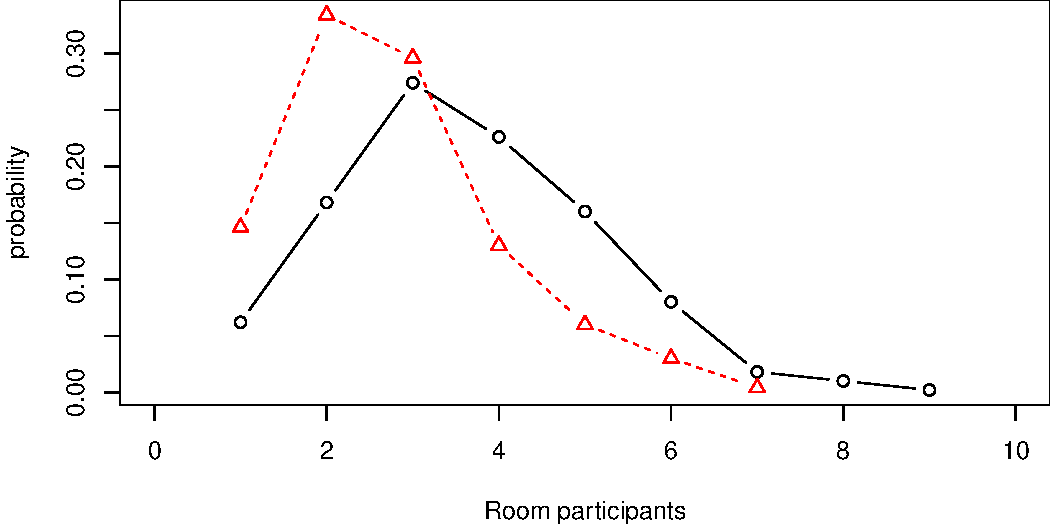
\includegraphics{report_notes_files/figure-latex/unnamed-chunk-2-1.pdf}
\caption{Simulated distribution of participants with uniform
distribution. Parameters are \(\eta=0.1\) and \(n=15\). Data simulated
500 times. Dashed curve had higher costs (\(x_l=1.5\)) than the solid
curve (\(x_l=0.5\)).}
\end{figure}

\subsection{Example with Beta
distribution}\label{example-with-beta-distribution}

In this example, we assume abilities are drawn from a lognormal
distribution with parameters \(\mu\) and \(\sigma\).

\section{Estimation}\label{estimation}

Our aim is to estimate the parameters \(\theta\) and \(\beta\) and to
evaluate whether costs are different between the three competition modes
under study: race, tournament, tournament + requirement.

It is natural to estimate the parameters \(\theta\) by maximum
likelihood because the ability distribution (and therefore the
distribution of the outcomes) is known. The estimation criterion used
here is the maximization of the \emph{deviance}.

The deviance is:

\begin{equation}
    D(\theta) = -2 \sum Y \log (\frac{N p(x, \theta)}{Y}) 
        + (N - Y) \log ( \frac{N - N p}{N - Y}).
\end{equation}

Note that the deviance is a function of the likelihood (see xxx pg.
xxx).

\begin{Shaded}
\begin{Highlighting}[]
\CommentTok{# Define likelihood}
\NormalTok{structreg <-}\StringTok{ }\ControlFlowTok{function}\NormalTok{(x, y, }\DataTypeTok{wt =} \KeywordTok{rep}\NormalTok{(}\DecValTok{1}\NormalTok{, }\KeywordTok{length}\NormalTok{(y)), }\DataTypeTok{intercept =} \OtherTok{TRUE}\NormalTok{, }\DataTypeTok{start =} \KeywordTok{rep}\NormalTok{(}\DecValTok{0}\NormalTok{, p), ...) \{}
\NormalTok{    fmin <-}\StringTok{ }\ControlFlowTok{function}\NormalTok{(beta, X, y, w) \{}
\NormalTok{        p <-}\StringTok{ }\DecValTok{1} \OperatorTok{-}\StringTok{ }\NormalTok{(beta }\OperatorTok\StringTok{ }\NormalTok{X)}\OperatorTok{^}\NormalTok{(}\DecValTok{1}\OperatorTok{/}\NormalTok{n)  }\CommentTok{# Function of parameters}
        \OperatorTok{-}\KeywordTok{sum}\NormalTok{(}\DecValTok{2} \OperatorTok{*}\StringTok{ }\NormalTok{w }\OperatorTok{*}\StringTok{ }\KeywordTok{ifelse}\NormalTok{(y, }\KeywordTok{log}\NormalTok{(p), }\KeywordTok{log}\NormalTok{(}\DecValTok{1}\OperatorTok{-}\NormalTok{p))) }
\NormalTok{    \}}
\CommentTok{#   gmin <- function(beta, X, y, w) \{}
\CommentTok{#       # Gradient here!}
\CommentTok{#   \}}
    \ControlFlowTok{if}\NormalTok{(}\KeywordTok{is.null}\NormalTok{(}\KeywordTok{dim}\NormalTok{(x))) }\KeywordTok{dim}\NormalTok{(x) <-}\StringTok{ }\KeywordTok{c}\NormalTok{(}\KeywordTok{length}\NormalTok{(x), }\DecValTok{1}\NormalTok{)}
\NormalTok{    dn <-}\StringTok{ }\KeywordTok{dimnames}\NormalTok{(x)[[}\DecValTok{2}\NormalTok{]]}
    \ControlFlowTok{if}\NormalTok{(}\OperatorTok{!}\KeywordTok{length}\NormalTok{(dn)) dn <-}\StringTok{ }\KeywordTok{paste}\NormalTok{(}\StringTok{"Var"}\NormalTok{, }\DecValTok{1}\OperatorTok{:}\KeywordTok{ncol}\NormalTok{(x), }\DataTypeTok{sep=}\StringTok{""}\NormalTok{)}
\NormalTok{    p <-}\StringTok{ }\KeywordTok{ncol}\NormalTok{(x) }\OperatorTok{+}\StringTok{ }\NormalTok{intercept}
    \ControlFlowTok{if}\NormalTok{(intercept) \{x <-}\StringTok{ }\KeywordTok{cbind}\NormalTok{(}\DecValTok{1}\NormalTok{, x); dn <-}\StringTok{ }\KeywordTok{c}\NormalTok{(}\StringTok{"(Intercept)"}\NormalTok{, dn)\} }
    \ControlFlowTok{if}\NormalTok{(}\KeywordTok{is.factor}\NormalTok{(y)) y <-}\StringTok{ }\NormalTok{(}\KeywordTok{unclass}\NormalTok{(y) }\OperatorTok{!=}\StringTok{ }\DecValTok{1}\NormalTok{)}
\CommentTok{#   fit <- optim(start, fmin, gmin, X = x, y = y, w = wt, method = "BFGS", ...)}
\NormalTok{    fit <-}\StringTok{ }\KeywordTok{optim}\NormalTok{(}\FloatTok{0.5}\NormalTok{, fmin, }\DataTypeTok{X =}\NormalTok{ x, }\DataTypeTok{y =}\NormalTok{ y, }\DataTypeTok{w =}\NormalTok{ wt, }\DataTypeTok{method =} \StringTok{"BFGS"}\NormalTok{, ...)}
    \KeywordTok{names}\NormalTok{(fit}\OperatorTok{$}\NormalTok{par) <-}\StringTok{ }\NormalTok{dn}
    \KeywordTok{cat}\NormalTok{(}\StringTok{"}\CharTok{\textbackslash{}n}\StringTok{Coefficients:}\CharTok{\textbackslash{}n}\StringTok{"}\NormalTok{); }\KeywordTok{print}\NormalTok{(fit}\OperatorTok{$}\NormalTok{par)}
    \KeywordTok{cat}\NormalTok{(}\StringTok{"}\CharTok{\textbackslash{}n}\StringTok{Residual Deviance:"}\NormalTok{, }\KeywordTok{format}\NormalTok{(fit}\OperatorTok{$}\NormalTok{value), }\StringTok{"}\CharTok{\textbackslash{}n}\StringTok{"}\NormalTok{) }
    \KeywordTok{cat}\NormalTok{(}\StringTok{"}\CharTok{\textbackslash{}n}\StringTok{Convergence message:"}\NormalTok{, fit}\OperatorTok{$}\NormalTok{convergence, }\StringTok{"}\CharTok{\textbackslash{}n}\StringTok{"}\NormalTok{)}
    \KeywordTok{invisible}\NormalTok{(fit)}
\NormalTok{\}}

\CommentTok{# Create data }
\NormalTok{ilogit <-}\StringTok{ }\ControlFlowTok{function}\NormalTok{(x) }\KeywordTok{exp}\NormalTok{(x)}\OperatorTok{/}\NormalTok{(}\DecValTok{1}\OperatorTok{+}\KeywordTok{exp}\NormalTok{(x))}
\NormalTok{n <-}\StringTok{ }\DecValTok{50000}
\NormalTok{competitors <-}\StringTok{ }\DecValTok{5}
\NormalTok{x1 <-}\StringTok{ }\KeywordTok{rchisq}\NormalTok{(competitors, }\DataTypeTok{df=}\DecValTok{3}\NormalTok{)}
\NormalTok{x2 <-}\StringTok{ }\KeywordTok{runif}\NormalTok{(n)}
\NormalTok{x3 <-}\StringTok{ }\KeywordTok{rnorm}\NormalTok{(n)}
\NormalTok{X <-}\StringTok{ }\KeywordTok{cbind}\NormalTok{(}\KeywordTok{rep}\NormalTok{(}\DecValTok{1}\NormalTok{, }\KeywordTok{length}\NormalTok{(x1)), x1, x2, x3)}
\NormalTok{betas <-}\StringTok{  }\KeywordTok{c}\NormalTok{(}\OperatorTok{-}\FloatTok{2.5}\NormalTok{, }\FloatTok{0.1}\NormalTok{, }\FloatTok{0.25}\NormalTok{, }\FloatTok{0.5}\NormalTok{)}
\NormalTok{fc <-}\StringTok{ }\KeywordTok{ilogit}\NormalTok{(X }\OperatorTok\StringTok{ }\NormalTok{betas) ## This the fixed cost}
\NormalTok{p <-}\StringTok{  }\DecValTok{1} \OperatorTok{-}\StringTok{ }\NormalTok{fc}\OperatorTok{^}\NormalTok{(}\DecValTok{1}\OperatorTok{/}\NormalTok{competitors) }
\NormalTok{y <-}\StringTok{ }\KeywordTok{rbinom}\NormalTok{(}\DataTypeTok{n=}\NormalTok{n, }\DataTypeTok{size=}\NormalTok{competitors, }\DataTypeTok{prob=}\NormalTok{p)}

\CommentTok{# Objective function}
\NormalTok{fmin <-}\StringTok{ }\ControlFlowTok{function}\NormalTok{(beta, X, y, w, competitors) \{}
\NormalTok{    p <-}\StringTok{ }\DecValTok{1} \OperatorTok{-}\StringTok{ }\KeywordTok{ilogit}\NormalTok{(X }\OperatorTok\StringTok{ }\NormalTok{beta)}\OperatorTok{^}\NormalTok{(}\DecValTok{1}\OperatorTok{/}\NormalTok{competitors)  }\CommentTok{# Function of parameters}
    \OperatorTok{-}\KeywordTok{sum}\NormalTok{(}\DecValTok{2} \OperatorTok{*}\StringTok{ }\NormalTok{w }\OperatorTok{*}\StringTok{ }\KeywordTok{ifelse}\NormalTok{(y, }\KeywordTok{log}\NormalTok{(p), }\KeywordTok{log}\NormalTok{(}\DecValTok{1}\OperatorTok{-}\NormalTok{p))) }
\NormalTok{\}}

\NormalTok{b.start <-}\StringTok{ }\KeywordTok{runif}\NormalTok{(}\KeywordTok{length}\NormalTok{(betas))}
\NormalTok{(out <-}\StringTok{ }\KeywordTok{optim}\NormalTok{(b.start, fmin, }\DataTypeTok{X=}\NormalTok{X, }\DataTypeTok{y=}\NormalTok{y, }\DataTypeTok{competitors=}\NormalTok{competitors, }\DataTypeTok{w=}\KeywordTok{rep}\NormalTok{(}\DecValTok{1}\NormalTok{, }\KeywordTok{length}\NormalTok{(y)))}\OperatorTok{$}\NormalTok{par)}
\end{Highlighting}
\end{Shaded}

\begin{verbatim}
## [1] -12.9291781   0.4352842   0.8931060   2.0707229
\end{verbatim}

\begin{Shaded}
\begin{Highlighting}[]
\KeywordTok{rbind}\NormalTok{(out}\OperatorTok{/}\NormalTok{competitors, betas)}
\end{Highlighting}
\end{Shaded}

\begin{verbatim}
##            [,1]       [,2]      [,3]      [,4]
##       -2.585836 0.08705684 0.1786212 0.4141446
## betas -2.500000 0.10000000 0.2500000 0.5000000
\end{verbatim}

\subsection{More examples}\label{more-examples}

Suppose F is lognormal(\(\mu, \sigma\)), then the zero profit condition
is:

\begin{align}
    \left[\frac 12 +\frac 12 \left(\frac{\log{\mtype}-\mu}{\sqrt{2\sigma}}\right)\right] = a^{-1/(n-1)} K_l
\end{align}

\begin{verbatim}
# xxx
zeroprofit <- function(x, mu, sigma, n) {
    x * plnorm(x, meanlog=mu, sdlog=sigma)^(n-1)
}
for (i in 3:10)
    curve(zeroprofit(x, i, 10, 10), add=TRUE, lty=i)
\end{verbatim}

\bibliography{library.bib}

\end{document}